\section{Methodology}\label{secmethodology}
In this section, the way in which the project was planned, organised, managed and decisions made throughout its life cycle will be discussed. Initial research and decisions regarding the team's approach to this project will be examined, before detailing any differences in the way in which this project ultimately panned out.

\subsection{Preliminary Research and Project Commencement}\label{prelim}
The team had their first meeting in late September, shortly after specifications for the project and dissertation had been given. It was agreed that getting started as soon as possible was best, and an agreement was reached to decide on an idea and carry out some research before starting any of the applied aspects of the project. 

While the team had a number of basic possible concepts which would be suitable for the scope of a final year project, taking on a data analytics project in the form of analysing cryptocurrency was considered to be the most interesting. The team had also agreed that machine learning should be incorporated into the project if possible, and saw pursuing this idea as an opportunity to include some innovative machine learning technologies in an interesting and relevant way. It was decided that a web application containing graphs of currency prices and a future price prediction feature would be ideal for this purpose and to demonstrate all theoretical aspects of this project, which would be discussed in the dissertation.

Following this decision, the first meeting with the team's supervisor was organised, in which all ideas were discussed. It was agreed that a cryptocurrency data analytics project would be a suitable and interesting project, and the team were given advice as to what technologies should be considered for use. Taking this advice on board, the team began more detailed research.

\subsubsection{Research Methodology}\label{secresearchmeth}
As all team members had some previous experience with cryptocurrency, it was agreed that major preliminary research into the concept was not a requirement. The team did some light reading of the latest news items relating to cryptocurrency and moved on to researching a list of technologies, examining which would be best to include in the applied project.

\textbf{\textit{Database of Prices:}} Based on the team's collective experiences from the previous academic year, it was first agreed that \textit{Python 3} would be ideal for obtaining data. The team carried out some quick searching online and found there to be numerous free cryptocurrency APIs (\textit{Application Programming Interfaces}) available, all of which stored vast amounts of records for prices of cryptocurrency against a variety of traditional currencies for increments of time, usually every minute. The team concluded this was often enough for a web application which does not deal with trading and therefore does not need to be accurate. After refreshing collective knowledge of MongoDB documentation \cite{mdbdocs}, the team agreed on using a MongoDB database to save data into from an API via a Python 3 script.

\textbf{\textit{Web Application Back-End:}} Having decided the details of the project's database system, the team began discussing the back-end of the application. Once again, previous experiences encouraged the use of Python 3 and the Flask Framework. All team members had enjoyed using this combination for previous web application projects, and felt it would simply make sense to do so again.

\textbf{\textit{Web Application Front-End:}} Based on the advice of the team's supervisor, research on \textit{Vue.js} \cite{vuejs} and \textit{D3.js} \cite{d3js} was carried out. It appeared this combination would work well for creating a web application with simple yet intuitive design, as well as creating striking visual representations of our data.

\textbf{\textit{Web Application Hosting:}} During prelimary research, the team considered both Microsoft Azure \cite{azure} and Heroku \cite{heroku} for deployment of the final application. Having deliberated over the technologies for some time, the team considered using Microsoft Azure due to previous experience and its vast quantity of features, all of which could be confidently relied on. However, it was noted that this was not a definite decision at the time, and the team were still open to the possibility of using Heroku if it were more suitable when the time came to deploy the application.

\textbf{\textit{Containerisation:}} Having heard about the benefits of containerisation, the team researched Docker \cite{docker}, a leading platform in containerisation. Containerisation, put simply, is the packaging of applications \textit{with} all relevant libraries and dependencies. This feature eliminates issues when trialling applications on different machines which may arise due to conflicts in installed software and the software the application was initially built with. While this was not a crucial element to the project, it would be convenient to implement should any related problems arise.

\textbf{\textit{Machine Learning:}} With regards to attempting to decipher trends in prices, the team's supervisor recommended the use of TensorFlow \cite{tensorflow}. Having been using this machine learning framework in class for some time at this point, the team were familiar with the framework and had been using the technology with Python 3. It was agreed that this combination should be used, as it would fit in well with the overall project architecture.

\subsubsection{Initial Expected Architecture}
Based on the research described above, the architecture depicted in \textit{Figure \ref{initarchitecture}} was decided upon. Of course, no aspect of this architecture was a concrete decision as the team felt it necessary to allow for discovery of new, possibly more suitable technologies.

\newpage

\begin{figure}[h]
    \centering
    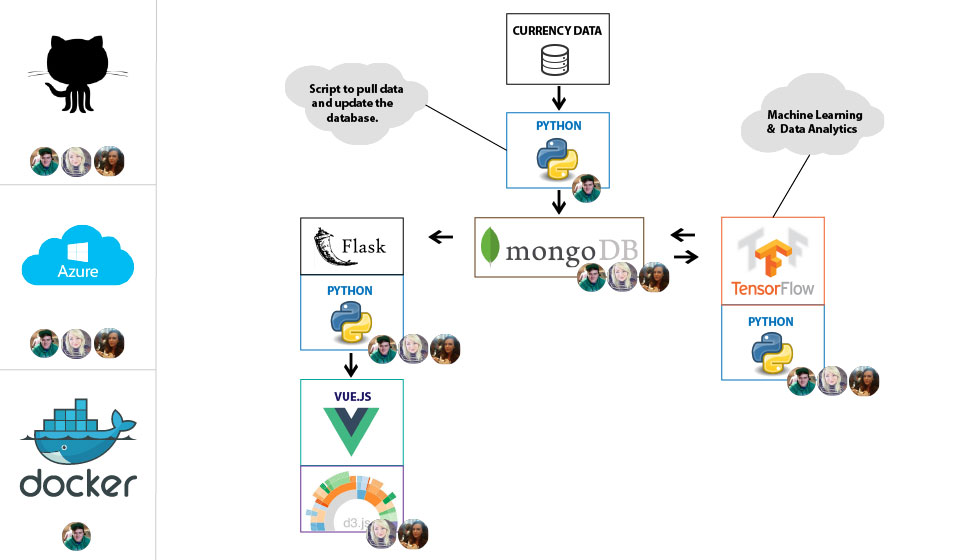
\includegraphics[width=0.9\textwidth, keepaspectratio]{img/Architecture.jpg}
    \caption{Planned Architecture, \textit{October 2017}}
    \label{initarchitecture}
\end{figure}

\subsubsection{Agile Development}
Having learnt about the various approaches to software development in previous academic years, the team felt that the \textit{Agile Methodology} \cite{agilemani} was the best to follow. In \cite{agileieee}, Highsmith et al highlighted the attractiveness of the agile approach, stating that working code and a team who work together effectively are the two main concepts stressed in agile methods \cite{agileieee}; working code proves to both developers and clients exactly what has been done, and an effective team can achieve cost savings as well as flexibility. Regular interaction between team members and the closeness of a team are also fundamental to agile methods, further pointed out by Highsmith in \cite{agileieee}. The team agreed this was the ideal methodology to follow, as regular communication and a stable, consistent timeline of work were strongly desired. 

Agile approaches often include the division of work into short periods of time called sprints, often a two to six weeks in length. At the beginning of each sprint, a goal for the end of the sprint is defined, such as a particular component of the project to be working, or some element to have been tested extensively. It was agreed that the inclusion of four week sprints in this project's life cycle would further help the team to keep on top of the project workload, providing a definitive timeline of progress.

\subsubsection{Version Control}
Having used free online version control software GitHub for a number of years, the team decided it would be ideal for keeping track of source code throughout this project. One particularly useful feature of GitHub is branches, allowing users to push to a given repository without necessarily affecting the original master branch. The team intended to have a branch for each member's work, a branch for developing (where individual work would be tied together), a branch for testing, a branch for machine learning, and a branch for dissertation work. Workload was divided between the team members as follows:

\begin{itemize}
    \item Tara O'Kelly: Front-End Development, including visualising currency data on a graph.
    \item Johnny Glynn: Back-End Development, including obtaining and saving currency data.
    \item Rebecca Kane: Dissertation, including relevant research.
\end{itemize}

It was decided that it would be best if the team worked collectively on any machine learning elements after the work specified above was complete, and thus didn't initially allocate it to any one member. 

It was acknowledged that GitHub's \textit{Issues} feature would come in very useful for keeping track of any problems. The team planned to use this to organise both technical code-related issues and issues related to the dissertation, such as information being required from one member or another on a particular subject or technology.

GitHub's \textit{Projects} resource would also add to the overall organisation of the project. \textit{Projects} are very similar to to-do lists and can be used in conjunction with Issues, allowing to-do items to be assigned to certain members. GitHub allows the creation of multiple \textit{Projects}, meaning one could be created for each major component of this project, such as Dissertation or Machine Learning.

\subsubsection{Testing}
It was agreed by the team that in keeping with the metrics discussed in \textit{\ref{metrics}: Metrics for Success or Failure}, testing should be user driven for the most part. Based on the metrics outlined in the aforementioned section, the team decided on the following tests related to each metric: 

\begin{itemize}
    \item\textit{Metric One - Easily understood, cohesive dissertation}: In order to test whether the team had succeeded in providing a clear and comprehensive examination of cryptocurrency in this dissertation, the team agreed it was best to ask those who had little or no understanding of cryptocurrency to read Chapters \textit{\ref{understandingcryptocurrencych}: Understanding Cryptocurrency} and \textit{\ref{predictingpricesch}: Predicting the Prices of Cryptocurrency}. It was decided that those who read the chapters would be asked to rate how well they understood the content on a scale of one to five, with one being no understanding and five being perfectly understood. The team agreed a test sample size of five or six people would suffice.
    \item\textit{Metric Two - Simple Web Application}: Again, it was decided that in order to test the simplicity of the web application, it would be best to ask those who had little or no knowledge of cryptocurrency. Similar to the above, five users would be asked to use the web application for a brief period of time and provide feedback on their opinions of its usability, using the same scale as above.
    \item\textit{Metric Three - Future Cryptocurrency Price Estimates}: In order to test the accuracy of the web application's predictions, it was agreed that the predictions should be tested over a period of one week, or seven predictions. Due to TensorFlow's training and testing facilities, this test could be carried out in one sitting. The TensorFlow model would be trained, and subsequently shown seven unseen prices, and asked to predict the new price. For example, the model can be shown a price from 11 December 2017 and asked to predict the price for the following day, which can then be compared against the actual data from 12 December 2017.
    \item\textit{Metric Four - Teamwork}: Of course, teamwork is not something which can be measured in a definitive way. It was determined that in order to measure the success of this, the team would simply reflect at the conclusion of this project on how issues were resolved, and if relationships were affected by any disagreements. 
\end{itemize}

\subsubsection{Supervisor Meetings}
During the first meeting with the team's supervisor, it was discussed what the frequency of supervisory meetings should be. The collective feeling was that a weekly meeting would be too often, as some weeks would naturally allow for more or less work to be done than others. It was determined that it was best not to have meetings if a substantial amount of work had not been done, and it was concluded that meetings would be best if only had when warranted, ideally every few weeks.

\subsection{Issues Encountered During the Development Process}\label{issuesencountered}
While the team initially had great intentions and did begin work on this project as soon as requirements were available, numerous issues ultimately surfaced.

\subsubsection{Interfering Factors}
Of course, at certain stress points throughout the academic year, work on this project was postponed due to upcoming exams or deadlines related to the team's other projects. As the first semester of this year involved more modules and therefore more work than the second semester, the collective decision was made by the team to put other projects first from late November 2018 through to early January 2018, when the second semester began. However, significant progress was made by the team between September and the end of November and this decision was believed to not have seriously jeopardised the progress of this project. A supervisory meeting was arranged in late November to discuss the work achieved thus far, and again in early January to discuss the direction of the project from that point. After regular contact with the team's supervisor, work proceeded again from mid January onwards.

\subsubsection{Communication Issues}
While communication was not an issue in the first semester of this year, it quickly became a problem as one team member unfortunately became ill in late January 2018, and remained so for the rest of the duration of the project. Contrary to what Agile development encourages, the team began to rely on messages, emails and occasional phone calls in order to keep in contact with the absent member. This ultimately led to a strain on development, as it grew more and more difficult to express ideas, plan for subsequent work through messages and calls. As the Agile Manifesto states, \textit{"The most efficient and effective method of conveying information to and within a development team is face-to-face conversation"} \cite{agilemani}. The team fully supports this statement, as there was no comparison between discussing components of the project through practical examples in person, and trying to do the same simply over the phone. There were also a number of occasions where a meeting was agreed for a certain day and time, only to result in two members being present due to lack of communication.

These communication issues ultimately delayed development, as other team members had to wait on the absent member to publish work on GitHub or reply to messages, as opposed simply seeing each member's work in person, or talking face to face and having an immediate reply. 

\subsubsection{Lack of Working Code}
As mentioned in the previous section, one team member had become ill and was absent from late January onwards. The two remaining team members continued to work on research based elements for some time, as they required work from the ill member in order to progress properly with their own work. While we acknowledge that some work could have been done by the remaining members by assuming the work of the absent member had been done in a certain manner, any progress made by the remaining members would ultimately have had to have been altered to suit the absent member's work. This method likely would have resulted in integration problems closer to the deadline, and thus it was decided that we would wait for the absent member to publish their code on GitHub.

While the absent member reassured remaining members that work was being done, there had been a lack of published code on their behalf since the previous semester. Nearing the end of the project, the remaining members continued to request that they see working code on the basis of being unable to spend any more time not moving forward in development. 

\subsubsection{Resolution of Problems}
On the basis of the issues discussed above, two members of the team brought their concerns to the project supervisor to look for advice. The options of continuing along the same track with all members contributing to the one project, or a division of the group to work on two separate projects were presented to the team. A discussion was held between all three team members, and it was mutually agreed on 9 April 2018 that the option to work as two separate teams from then on was best for all members. Keeping in mind the teamwork objectives outlined in \textit{\ref{objectives}: Objectives} and \textit{\ref{metrics}: Metrics for Success or Failure}, the team agreed to not let any of these issues affect their friendships, and have succeeded in doing so thus far.

\subsubsection{Development Following Group Partition}
As there was little time left after the decision to separate into two groups, development in the last week of the project became somewhat erratic, following aspects of Extreme Programming development methodologies. The team could not afford to put large quantities of time into planning, and thus decided to only use a few hours to plan for what needed to be completed in the week ahead. 

\textbf{\textit{Extreme Programming:}} Based on the fundamentals of the Extreme Programming methodology, outlined by Wells in \cite{xp}, this methodology is successful partly due to its encouragement of developers adapting to change, sometimes late in the development life cycle. The loss of one team member could be considered difficult to adapt to so late in this project's life cycle, but the team decided to follow the principles of Extreme Programming closely in order to overcome this. The team decided to self-organise around the problem to solve it as quickly as possible \cite{xp} and began reallocating tasks based on their importance. Once tasks had been outlined the team kept Wells' summary of a successful Extreme Programming project in mind - \textit{communication, simplicity, feedback, respect, and courage}. Over the final week of the project, the team kept in near constant contact with each other, also regularly discussing various facets of the project with their fellow students. Of course, at such a late stage the design of any further implementations must be as simple and clean as possible, a concept the team strived towards. Rather than test numerous implementations and methods, the team decided it best to research possible solutions to any problems, before implementing them. Ultimately, this saved much time, as a chosen solution was subsequently well understood and highly likely to work as expected. Finally, in keeping with initial objectives for this project, the team aspired to continuously be respectful in this time of high stress, while being courageous and trusting in their own decisions.

To conclude, the final week of this project was of course very demanding and stressful. One may have expected any work produced in this time frame to be cluttered, thrown together with haste in an attempt to meet deadlines. Fortunately, the quality of work by the team actually improved due to the crucial planning necessary in order to produce a large amount of work in such a short period of time.